%PART_1_CHAP_4
\myChapter[obotique, pédagogie et numérique]{R}{obotique, pédagogie~~\break et numérique}\label{sec:peda}
%WAIT a Review ok
\begin{resumChap}
Après avoir défini l'outil dans le chapitre 1, puis l'utilisateur et son contexte d'utilisation dans le chapitre 2, nous avons vu dans le chapitre 3 comment pouvait être définie la motivation.\par%
Dans ce quatrième chapitre, nous verrons quelles sont les caractéristiques inhérentes à la robotique et au numérique pouvant être exploitées à des fins pédagogiques.\par%
Principalement, nous aborderons le caractère tangible de ces objets, le rapport à l'erreur qu'offre la programmation de tels objets et comment l'enseignant doit se positionner dans ce contexte où l'information et le savoir sont directement accessibles par l'élève.\par%
Nous évoquerons également les principes de la méthode scientifique et de la déduction hypothético-déductive, démarche particulièrement pertinente pour l'utilisateur dans le contexte des activités robotiques que nous avons développé.
\end{resumChap}
\section{Un objet tangible}\label{sec:tangible}
    \paragraph{Définition}
        Dans le livre \cro{Le second soi - Les ordinateurs et l'esprit humain} de Sherry \citeB{turkle2005second}, le rôle social des \cro{jouets intelligents} est décrit comme des artefacts relationnels permettant aux enfants d'explorer \cro{la matière, la vie et l'esprit} \citeB{turkle2006encounters}. Pour Edith Ackermann, une psychologue qui a exploré les interactions entre la psychologie du développement, le jeu, l’apprentissage et la conception, les jouets animés sont des \cro{jouets qui font des choses} (\gui{\textit{playthings that do things}})~\citeB{ackermann2005playthings}. En jouant avec eux, les enfants sont véritablement amusés et intrigués par leur incongruité et les considèrent comme des amis.
        D'après le \sht{TLFI}, tangible provient de tangere qui signifie \gui{palpable} - \gui{Qui est perceptible par le toucher}.
        Une définition plus complète de tangible est fournie par le dictionnaire de Cambridge:
        \citeAtion{tangible-Cambridge}
        Réel et non imaginaire; capable d'être montré, touché ou expérimenté. 
        Le tangible est quelque chose, c'est la matière, c'est quelque chose de palpable qui donne des sensations. Cela peut être un objet. Il s’agit d’un effet physique car manipulé. Des informations sensorielles physiques sont ressenties, mais elles ont également une dimension cognitive car elles affecteront la perception et les émotions de l’utilisateur face à l’objet et à son environnement. En fonction de la nature de ses émotions et perceptions, l'attitude de l'utilisateur à l'égard de l'objet et de la situation sera modifiée.   
    \paragraph{Type d'interaction}
        Un \sht{tui} est une interface qui permet à l'utilisateur d'interagir avec des informations numériques via l'environnement physique. Ces actions de l'utilisateur peuvent être réalisées grâce à des objets physiques également appelés \cro{tokens}. Ils sont la représentation physique d'une information virtuelle. Eva Hornecker, 
        %professeure à l'Université du Bauhaus de Weimar, en Allemagne, 
        définit les \sht{tui} comme un moyen de créer une immersion dans l'expérience. Il peut soutenir la cognition spatiale des utilisateurs, réduire la charge cognitive et permettre une immersion plus créative dans le problème. Les actions qui se déroulent dans l'espace réel ont un parallèle virtuel~\citeB{hornecker2004tangible}.
        \begin{figure}[!h]
            \centering
            \label{fig:type_interac}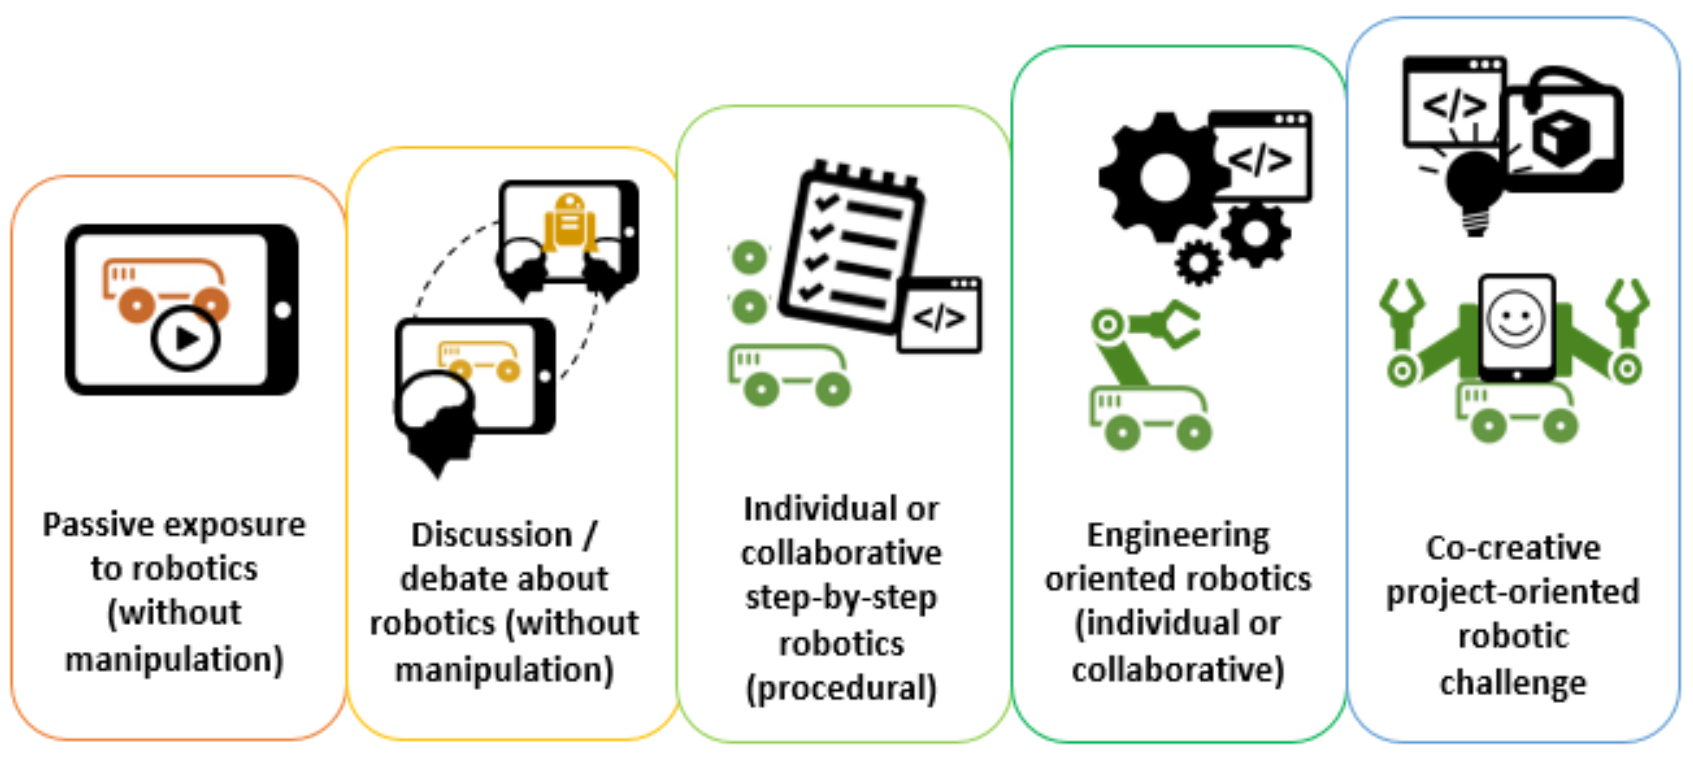
\includegraphics[width=\linewidth]{Figures/Romero-type_of_interac.png}
            \caption{5 types d'usages du numérique \citeB{romero2016educational}}
        \end{figure}\par%
        Les matériaux tangibles sont un facteur clé pour l'apprenant. Les travaux de Freinet~\citeB{freinet1969pour}, Montessori~\citeB{montessori2013montessori} et Alvarez~\citeB{alvarez2016lois}~\citeS{sec:peda_edu} montrent qu'avoir un objet spécifique à manipuler pour se concentrer sur une tâche donnée donne à l'apprenant une autonomie, lui permet de corriger ses erreurs et de comprendre les concepts abstraits qui se cachent derrière. 
    \paragraph{Impact sensoriel}
        %Nous savons que l'haptique est un phénomène complexe. Lors de tâches de manipulation d'objets, 
        Le cerveau sélectionne des éléments internes et externes spécifiques pour fixer son attention et évaluer ses performances sur les tâches qu'il exécute. Le signal reçu (type d'afférence et propriétés de réponse) reposera sur l'innervation sensorielle tactile de la main~\citeB{johansson2009coding}. Lederman~\citeB{lederman2009haptic} a décrit six \gui{procédures exploratoires} manuelles de manipulation tangible permettant d’examiner les propriétés d’objets suivants: texture, poids, dureté, volume, température et forme globale. Abraira~\citeB{abraira2013sensory} décrit les propriétés anatomiques et physiologiques des mécanorécepteurs à seuil bas, la comparaison particulière des sous-types de mécanorécepteurs cutanés ainsi que leurs propriétés et localisations de réponse, mais également leur stimulus optimal (étirement, vibration, déviation du follicule pileux, \etc). Puisqu'il existe différentes manières d'interagir par le toucher, la saisie, les sensations haptiques et la manipulation, il peut être intéressant d'explorer les émotions générées. McGlone~\citeB{mcglone2014discriminative} étudie le \textit{toucher affectif}. Il montre qu'un pinceau doux caressant la peau, active les zones somatosensorielles S1 et S2 ainsi que le cortex insulaire controlatéral postérieur. Le cortex insulaire est une région de grand intérêt pour les mécanismes affectifs et est considéré comme une passerelle entre les systèmes sensoriels et les systèmes émotionnels du lobe frontal~\citeB{augustine1996circuitry}. On pense également qu'il joue un rôle dans diverses fonctions liées à des émotions telles que l'empathie, la perception ou la conscience de soi et à la régulation de l'homéostasie du corps~\citeB{damasio2012persistence}.
    \paragraph{Impact Pédagogique}
        Lorsqu'il s'agit d'intégrer la théorie appliquée aux objets à manipuler, il est bon de garder à l'esprit les références précédentes, en particulier pour rappeler que la manipulation tangible d'objets peut avoir un impact sur la perception. Dans leur document intitulé \cro{Tangible Bits}, Ishii~\citeB{ishii1997tangible} décrit un moyen intelligent d’intégrer des interfaces concrètes dans la vie quotidienne des utilisateurs avec des avantages qui sont des possibilités d’actions sur les objets~\citeB{gibson1977theory}. Saisir et manipuler des objets permet aux utilisateurs de centrer leur attention sur ces objets physiques.
\section{Le rapport à l'erreur}\label{sec:erreur}
    Afin de laisser la plus grande autonomie possible à l'apprenant, le support doit être auto-correctif et spécifique, car comme le soulignait Freinet~\citeB{freinet1969pour}; l'élève reste l'élément central, l'enseignant est présent en tant qu'instigateur de l'activité qu'il devra sélectionner, d'après Montessori~\citeB{montessori2013montessori}, dans le respect des périodes sensibles de l'apprenant. Dès lors, il pourra distinguer les notions, les préciser, les généraliser, du concret vers le concept et du concept vers l'abstrait. 
    Le robot reste un support pédagogique rendant attrayant l'apprentissage d'un langage de programmation car il permet à un étudiant, programmant le robot puis observant son comportement, d'avoir un retour direct sur ce qu'il a écrit.
\section{Le rôle de l'enseignant}
    \paragraph{Adapter les ressources} 
        La robotique est largement pluri-disciplinaire~\citeS{sec:pluri_bot}. De plus, la robotique peut être vue comme un moyen (un outil) ou une fin (apprendre la robotique). Les plateformes sont plus ou moins libres~\citeS{sec:open}, et donc plus ou moins détournables~\citeS{sec:re-use}. L'enseignant doit donc, dans un premier temps, déterminer les objectifs théoriques: les connaissances et compétences à acquérir \tiret{relevant de la robotique~\citeS{sec:concept}, ou non} puis, dans un second temps, les moyens pédagogiques~\citeS{sec:peda_edu} les plus adaptés à son public, sa classe, pour la garder motivée~\citeS{sec:motiv}. Il doit ensuite sélectionner parmi les ressources disponibles~\citeS{sec:bot} celles qu'il trouve pertinent d'intégrer à sa pratique de manière totale ou partielle. De là, il développera son propre matériel pédagogique, ses propres histoires.
    \paragraph{le storitelling}\label{sec:storitell}
        Le storytelling est une technique de communication visant à stimuler le lecteur en le faisant rentrer dans une histoire, un récit, qui illustre et rend tangible un problème donné. Mais le storytelling a une finalité, transmettre un message le plus souvent par des méthodes de persuasion. Ce process passe par une captation de l'attention, la stimulation (ou la création) d'un désir chez l'auditeur puis par l'argumentaire d'une solution. Cette technique s'éloigne drastiquement du triptyque de communication classique: identification / analyse / résolution. 
        Dans notre cadre, il s'agit avant tout de mise en scène et d'illustration de notions et non pas de stratégie de communication comme Steve Denning~\citeB{denning2005mastering}, l'un de ses premiers théoriciens.\par%
        Donner un objectif final, un prétexte, à la réalisation de la tâche permet de la justifier. De plus, cela permet de diviser la tâche en différents sous objectifs et d'impliquer l'ensemble de la classe dans une cause commune, \cro{une même aventure}.  Souvent sous la forme d'un problème à résoudre, le travail peut être ensuite réalisé de façon individuelle ou collective et avec un mode coopératif ou compétitif. Par défaut, \cad sauf dans les contextes imposant des contraintes particulières, les activités coopératives de groupe sont plus pertinentes à mettre en place, et grâce au \sht{TIC} ces activités peuvent prendre une dimension internationale: simplement entre deux classes~\citeS{sec:prof-GL} ou mise en place par des organismes via des projets clé en main, comme avec le projet R2T2: \textit{en 2032, une météorite a endommagé une station d'approvisionnement d'énergie sur Mars!}
        \begin{figure}[!h]
        \begin{minipage}{0.475\linewidth}
            \centering
            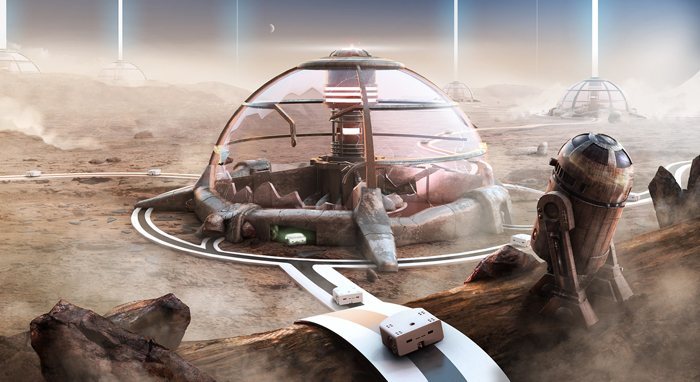
\includegraphics[width=\linewidth]{Figures/thymio-r2t2.jpg}
            \caption[\textit{ill.} Mission R2T2]{\textit{ill.} Mission R2T2~\citeURL{thymio_r2t2}}
            \label{fig:r2t2}
        \end{minipage}
        \hfill
        \begin{minipage}{0.475\linewidth}
        \myDefautStyle
            \gui{Nous devons évaluer les dégâts et remettre en marche le générateur principal. Nous avons 16 robots sur Mars, aux entrées de la station. Chaque robot peut être contrôlé par une équipe d'ingénieurs et de spécialistes depuis la terre.}~\citeURL{thymio_r2t2}.
            \newline\vfill
        \end{minipage}
        \end{figure}{}\par%
        C'est donc 16 équipes de différentes écoles, composées de 5 à 6 élèves entre 10 et 14 ans, qui sont invitées à remplir indépendamment plusieurs missions afin d'atteindre un objectif commun.
    \paragraph{Gestion de l'effort}
        La gestion de la motivation intrinsèque de l'individu est essentielle. Les motivations extrinsèques ayant montré leurs limites particulièrement dans le monde de l'éducation.
        C'est bien l'intérêt et le plaisir que porte l'apprenant sur son apprentissage qui va déterminer sa capacité à intégrer des nouveaux concepts, et non la pression sociale, les punitions ou les récompenses. Ainsi avoir recours aux nouvelles technologies dans ces enseignements permet de générer une force motivationnelle non négligeable. Cependant celle-ci est éphémère~\citeS{sec:honeyBee}. Renouveler ces enseignements pour offrir des ressources en adéquation avec les enjeux actuels de la société semble un bon moyen de garder l'élève intéressé, et donc motivé.
\section{L'interaction directe avec le savoir}\label{sec:mooc}
        \begin{figure}[!h]
          \begin{minipage}{0.45\linewidth}
              \centering
              \label{fig:triangle}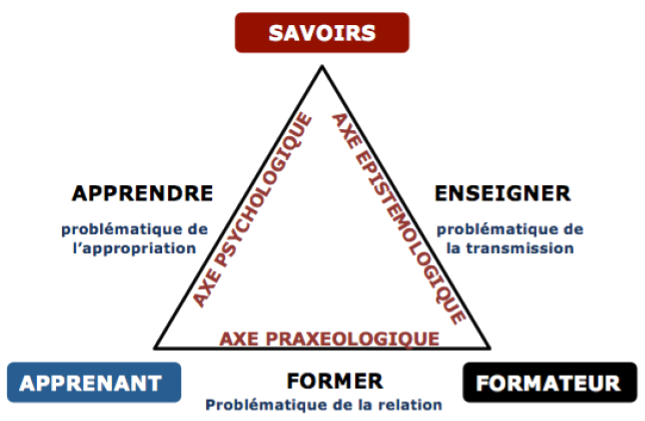
\includegraphics[width=\linewidth]{Figures/Houssaye-triangle.png}
              \caption{Triangle de la pédagogie, Houssaye~\citeB{houssaye1992triangle}}
          \end{minipage}
          \hfill
          \begin{minipage}{0.45\linewidth}
              \centering
              \label{fig:tetra}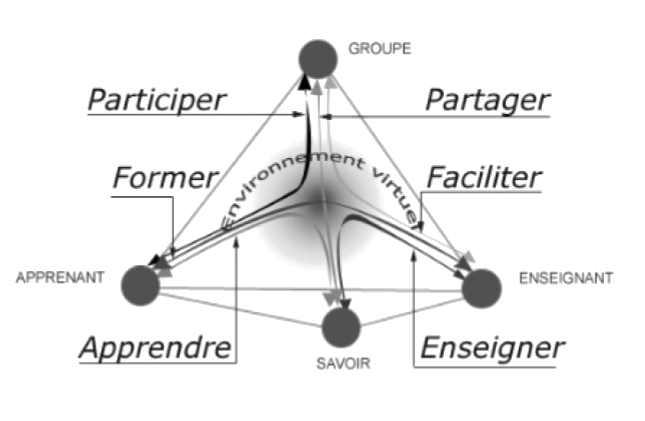
\includegraphics[width=\linewidth]{Figures/Faerber-tetra.png}
              \caption{Tétraèdre de la pédagogie, Faerber~\citeB{faerber2003groupements}}
          \end{minipage}
          \hfill
        \end{figure}\par%
        Les diagrammes présentés ci-dessus cherchent à formaliser les relations et les enjeux des différents acteurs de l'apprentissage. De leurs interactions émergent les principaux concepts liés au processus d'acquisition des connaissances. Ces concepts permettent de rendre compte des problématiques mises en œuvre dans l'environnement scolaire et plus généralement dans tous les environnements dédiés à la transmission du savoir. 
    \paragraph{Le Triangle de la pédagogie}    
        Ce modèle~\citeB{houssaye1992triangle}, déjà largement commenté dans la littérature, met en avant les relations existantes entre les acteurs: il les définit en précisant le cadre théorique de référence et la problématique associée.
        Le formateur doit avoir un regard épistémologique sur le savoir à enseigner, pour pouvoir le reconstruire avec l'apprenant tout en gardant une certaine distance; l'élève devant être capable in fine d'être autonome et d'avoir le recul nécessaire pour appréhender le savoir par lui-même. Le savoir n'est pas ici simple objet, il n'a pas un rôle statique; le caractère dynamique de son évolution et de sa reformulation n'est pas neutre et reflète les différences d'interprétations entre les individus.
        Mais ce système, dans son ensemble, n'est pas non plus statique et le poids de chaque nœud varie dans le temps et selon les individus. Cette double variation se répercute alors sur l'intégralité du graphique.
        Ainsi Houssaye a développé sa théorie sur l'inégalité des poids entre acteurs. Dès lors il fit un descriptif théorique de 3 contextes exacerbés: chacun des contextes est vu comme au détriment de l'un des acteurs. Ceci aurait pour conséquence directe de privilégier le processus associé aux deux autres acteurs.
        Exemple si l'apprenant se trouve, comme le dit Houssaye, à ‘la place du mort qui joue le fou’ c'est alors l'arc entre savoir et formateur qui est exacerbé: ainsi le formateur se focalise sur la construction de son contenu en délaissant l'apprenant et la relation qu'il entretient avec, pouvant donner naissance à un sentiment de frustration ou d'insatisfaction chez l'apprenant qui s'exprimera par une opposition (\eg manque d'attention, de respect, \etc). 
        A l'inverse, si la relation exacerbée est \cro{formée} alors c'est au détriment du savoir qui devient secondaire. Les aides et appuis du formateur sont fréquents, l'apprenant a alors parfois du mal à situer l'état de ses compétences et à percevoir la structure globale du cours, celle-ci s'adaptant en permanence à lui.
        L'une des principales limites de ce modèle est qu'il ignore totalement la dynamique de groupe. De plus le développement des technologies numériques a, entre autre, permis un accès massif et libre au savoir par l'apprenant. De nouvelles méthodologies de travail ont pu émerger comme la collaboration massive via le partage des ressources et codes sources. La diffusion et la transmission font également parties des axes majeurs du développement des sciences du numérique. Notamment les \sht{MOOC} qui ont opéré une véritable révolution dans la possibilité pour l'apprenant de choisir ses enseignements et ce sans aucune contrainte.
    \paragraph{Le Tétraèdre de la pédagogie}
        Prendre en compte la dimension numérique est essentiel et c'est ce qu’a compris Faerber, en 2002, lorsqu'il réfléchit au concept de groupe relié par un environnement virtuel\citeB{faerber2003groupements}.
        C'est dans le cadre du projet ACOLAD que Faerber a développé ce graphique. Ce projet porte essentiellement une vision et un système d'enseignement à distance. Dans notre cadre, enseignant et apprenant ne sont pas en situation de télé-enseignement, cependant certaines ressources essentielles peuvent se trouver à distance.
        Savoir utiliser les outils de communication tels que les forums, ou savoir \cro{fouiller} la documentation sont des compétences essentielles de nos jours. Bien souvent gages d'autonomie, elles facilitent la progression dans l'acquisition d'autres compétences en faisant le lien entre les besoins de l'utilisateur et les ressources mises en ligne par la communauté.
        Par ailleurs l'enseignant garde une place entière dans ce système, il a un statut particulier et développe une véritable relation de proximité avec l'apprenant. Cela lui offre un point de vue privilégié. Ainsi grâce à l'observation et l'analyse qu'il peut avoir sur la situation, il est le plus à même d'adapter l'enseignement à l'apprenant.
    \paragraph{La démarche scientifique}
        \begin{figure}[!h]
            \centering
            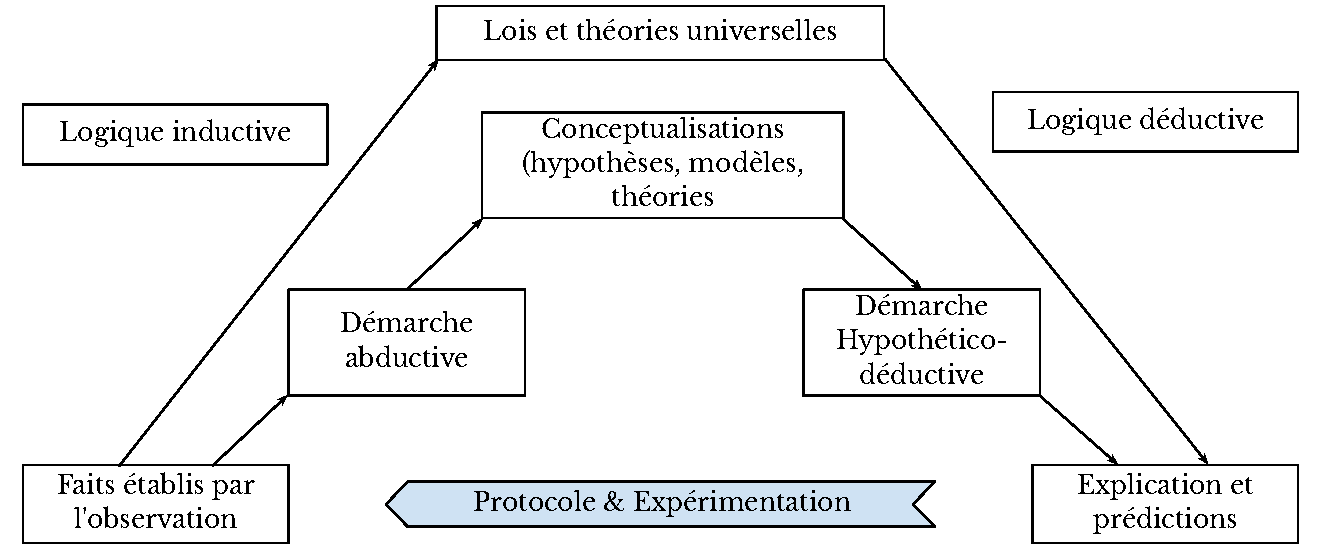
\includegraphics[width=\linewidth]{Figures/Bertacchini-methode-2015.pdf}
            \caption{Modes de raisonnement scientifique, Bertacchini~\citeB{Bertacchini2015methode}}
            \label{fig:methode}
        \end{figure}\nocite{atlan2019apprentissage}
      \subparagraph{La méthode scientifique}
        La méthode scientifique est souvent réduite à la seule approche hypothético-déductive, pourtant elle représente l'ensemble des pratiques devant guider le processus de production des connaissances scientifiques, qu'il s'agisse d'observations, d'expériences, de raisonnements, ou de calculs théoriques. Ainsi, \gui{\cro{la} méthode scientifique}, n'est pas unique malgré l'idée implicite que cette formulation peut véhiculer. Car, en effet, les pratiques des chercheurs se révèlent d'une si grande diversité de démarches et de disciplines scientifiques que l'idée d'une unité de la méthode est rendue très problématique. Cependant, plusieurs types \tiret{complémentaires} de modes de raisonnement peuvent être identifiés comme, par exemple, la logique déductive (du fait vers la théorie) et la démarche abductive (processus de généralisation par inférence) ou encore la logique inductive (de la théorie vers la prédiction, le fait) et la démarche hypothético-déductive.
      \subparagraph{L'approche hypothético-déductive}
        La démarche hypothético-déductive consiste à émettre une nouvelle hypothèse \tiret{cohérente dans le système de représentation déjà acquis pour l'individu}, puis, à partir de cette hypothèse, de générer une prédiction. Ce besoin de générer une nouvelle hypothèse est souvent associé à l'observation d'un fait nouveau devant être explicité, afin de résoudre un problème. On parle alors d'approche hypothético-déductive où la démarche éponyme est bouclée et associée à d'autres méthodes. En effet, il s'agit de réitérer une ou plusieurs expériences afin d'en extraire une loi générale à partir de l'observation et l'interprétation des résultats. Ces observations impliquent une première phase abductive en amont de la mise en place de la démarche hypothético-déductive et ce, en parallèle d'une méthode expérimentale permettant, par le recueil de données, de valider ou d'infirmer ces hypothèses initiales.
      \subparagraph{La méthodes expérimentales}
        Cette méthode a été centrale dans la révolution scientifique accomplie depuis le \siecle{17}, mais on retrouve ces traces dès le \siecle{1} de notre ère, avec le mathématicien Alhazen. Sa définition moderne est formulée par les français Michel-Eugène Chevreul, chimiste et le médecin Claude Bernard, en 1856~\citeB{chevreul1856lettres} et se voit résumée aujourd'hui ainsi pour le grand public:
        \citeAtion{methode}
        %Les méthodes expérimentales scientifiques consistent à tester la validité d'une hypothèse, en reproduisant un phénomène et en faisant varier un paramètre. Le paramètre que l'on fait varier est impliqué dans l'hypothèse, [\dots]~il s'agit de [le] modifier à l'aide d'un dispositif expérimental conçu pour permettre le contrôle de ces paramètres, dans le but de mesurer leurs effets et si possible de les modéliser.
        C'est exactement les méthodes que nous tentons de promouvoir dans la construction de nos activités. Notamment, en proposant des situations d'apprentissage propices à la progression par essai - erreur.